\begin{center}
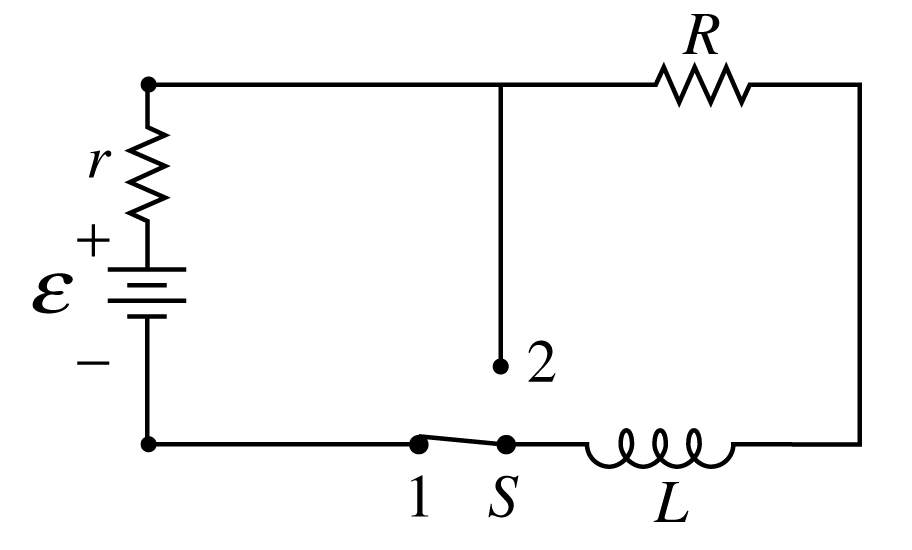
\includegraphics[scale=0.2]{images/img-010-017.png}
\end{center}

% Multiple Choice Question 19
\begin{questions}\setcounter{question}{18}\question
The circuit shown above consists of a battery of emf $\mathcal{E}$ and internal resistance $r$, a resistor $R$, an inductor $L$, and a switch $S$, initially in position 1. After the current $i$ in the inductor reaches its maximum value $I_{0}, S$ is switched instantaneously from position 1 to position 2 at time $t=0$. Subsequent variation of $i$ with $t$ is best represented by which of the following graphs?

\begin{oneparchoices}
\choice \adjustbox{valign=t}{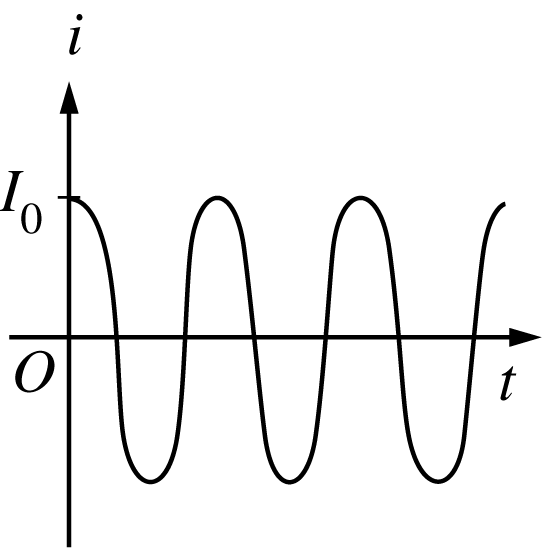
\includegraphics[scale=0.2]{images/img-010-018.png}}
\choice \adjustbox{valign=t}{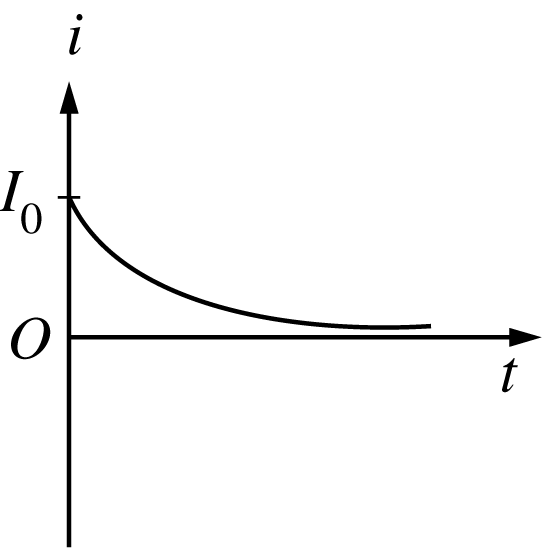
\includegraphics[scale=0.2]{images/img-010-019.png}}
\choice \adjustbox{valign=t}{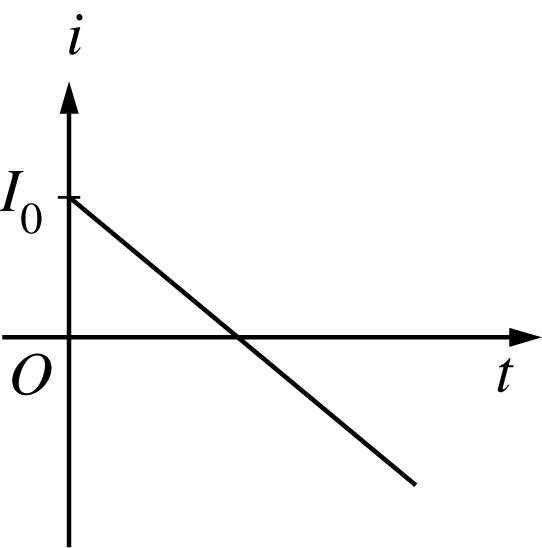
\includegraphics[scale=0.2]{images/img-010-020.png}}
\choice \adjustbox{valign=t}{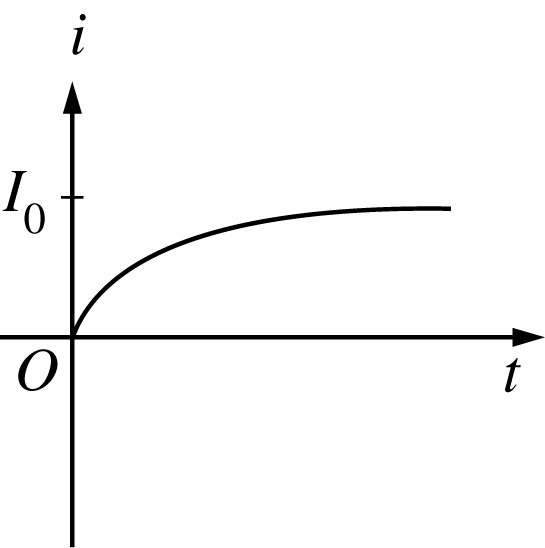
\includegraphics[scale=0.2]{images/img-010-021.png}}
\choice \adjustbox{valign=t}{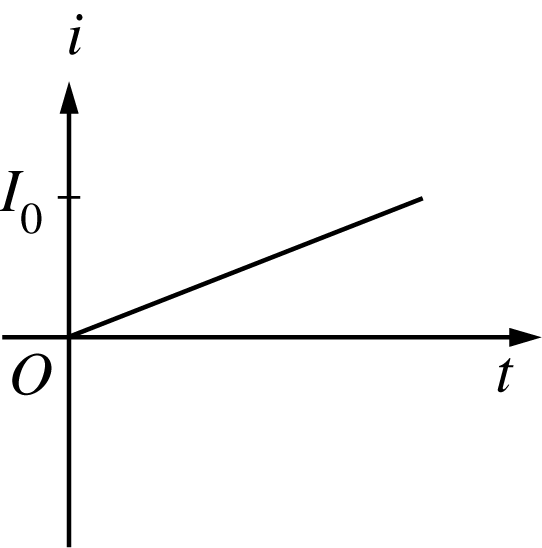
\includegraphics[scale=0.2]{images/img-010-022.png}}
\end{oneparchoices}\end{questions}

